%%%%% RESULTS %%%%%%
\section{Results}
\label{sec:results}

Figure \ref{fig:fidelity_plot} displays the haptic feedback fidelity and versatility scores of the systems described in each article. The quality score of each system is depicted by the dot's color and size, respectively (see section \ref{sec:quality}).


\subsection{Search Results}

%%%% Rewrite for precise numbers!! %%%%%

The search yielded 404 results, which were saved in the library of Mendeley. 75 duplicates were found and removed. The remaining 329 records were screened based on title and abstract first. This led to the preliminary exclusion of 290 records, of which 73 records were re-screened as they were from the years 2022-2024 (see fig. \ref{fig:prisma}), along with 3 papers that had been included based on citation search. 
65 records were excluded during this screening.

In total, 50 articles were eligible for the full-text screening. Of these, 14 were excluded based on the exclusion criteria, and the remaining 36 studies were included in this review.


\subsubsection{Study characteristics}
\paragraph{Year of publication}
The year of publication of the included studies ranges from 2000 to 2024. As seen in \ref{fig:years}, the number of studies has greatly increased in the past decade, with a peak in 2018.

\begin{figure}[htbp]
    \centering
    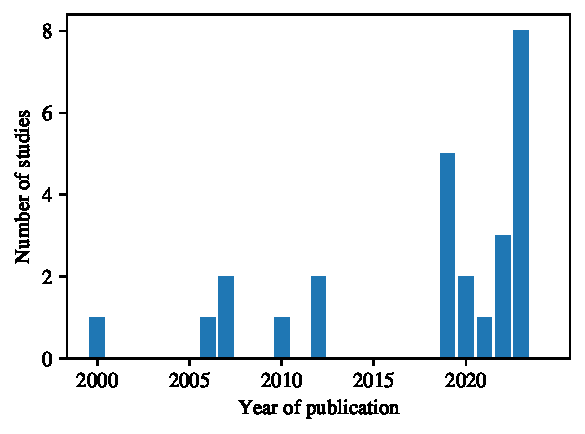
\includegraphics[width=\columnwidth]{figures/years.pdf} 
    \caption{Publication dates of the included articles}
    \label{fig:years}
\end{figure} 




\paragraph{Body parts involved}
% Graph to quantify involved body parts (pie chart)

Figure \ref{fig:body_parts_pie} shows which body parts were involved in the studies. As can be seen, most studies were concerned with stimuli at the palm and fingers, and many experiments also involved the forearm and upper arm. The fewest studies involved the feet, namely, the experiments with the DaVinci Research Kit \cite{Caccianiga2021, Oquendo2024}.

\begin{figure}[htbp]
    \centering
    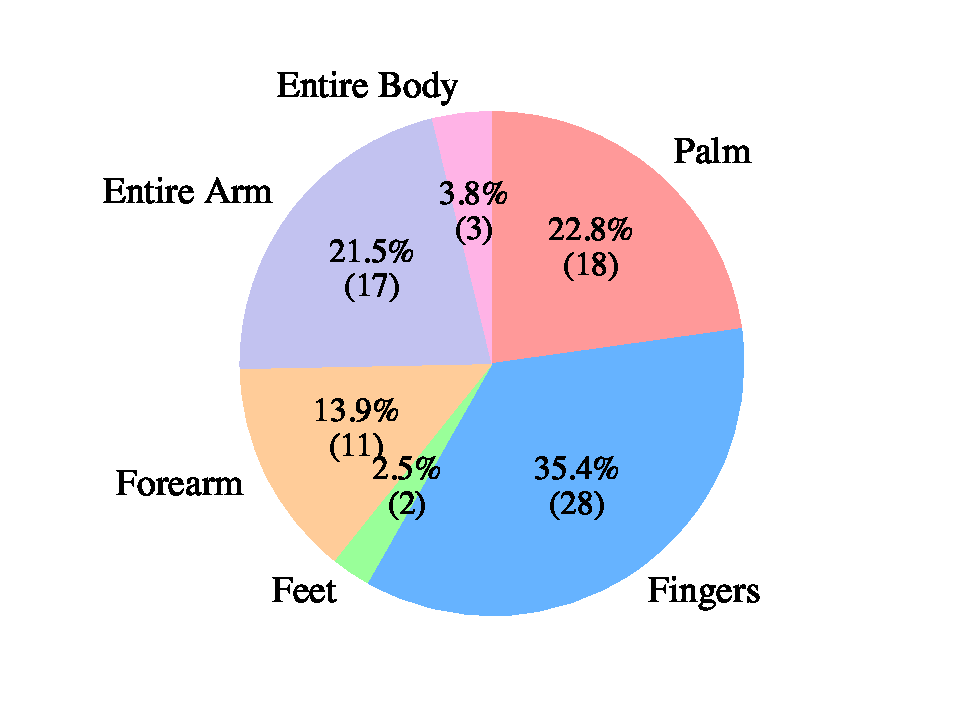
\includegraphics[width=\columnwidth]{figures/body_pie.pdf} 
    \caption{Body parts involved in the studies}
    \label{fig:body_parts_pie}
\end{figure} 


\begin{figure*}[htbp]
\begin{tikzpicture}[scale=3.6]
    
    % Add axis labels
    \foreach \x in {0,1,2,3,4} {
        \draw [very thin, lightgray](\x cm, 0-0.05) -- (\x cm, 4+0.05) node[anchor=north] {};
        \draw [very thin, lightgray](0-0.05,\x cm) -- (4+0.05,\x cm) node[anchor=east] {};
    }

    % Draw axes
    \draw[thick,<->] (0,2) -- (4,2) node[anchor=south west] {Haptic Fidelity};
    \draw[thick,<->] (2,0) -- (2,4) node[anchor=south] {Versatility};

    \node at (0,1.9) {\footnotesize{abstract}};
    \node at (4,1.9) {\footnotesize{realistic}};
    \node at (1.8,0.1) {\footnotesize{specific}};
    \node at (1.8,3.9) {\footnotesize{generic}};

    % Legend
    \draw[fill=white] (0.1,3.9) rectangle (1.2,3.25); % Legend border
    \node[anchor=west] at (0.15, 3.8) {\textbf{Legend}}; % Legend title
    
    \node[circle, fill=c1, inner sep=2.3pt] at (0.22, 3.65) {};
    \node[anchor=west] at (0.25, 3.65) {\footnotesize{Quality $q > 0.9$}};

    \node[circle, fill=c2, inner sep=2pt] at (0.22, 3.55) {};
    \node[anchor=west] at (0.25, 3.55) {\footnotesize{Quality $0.8 < q \leq 0.9$}};

    \node[circle, fill=c3, inner sep=1.7pt] at (0.22, 3.45) {};
    \node[anchor=west] at (0.25, 3.45) {\footnotesize{Quality $0.7 < q \leq 0.8$}};

    \node[circle, fill=c4, inner sep=1.4pt] at (0.22, 3.35) {};
    \node[anchor=west] at (0.25, 3.35) {\footnotesize{Quality $q \leq 0.7$}};
    
    % Sample data points
    \node[circle, fill=c1, inner sep=2.3pt] at (3.5,2) {};
    \node[circle, fill=c1, inner sep=2.3pt] at (3.22,2) {};
    \node[circle, fill=c1, inner sep=2.3pt] at (0.63,2) {};
    \node[circle, fill=c1, inner sep=2.3pt] at (3.38,2) {};
    \node[circle, fill=c1, inner sep=2.3pt] at (3.75,2) {};
    \node[circle, fill=c1, inner sep=2.3pt] at (2.63,2) {};
    \node[circle, fill=c1, inner sep=2.3pt] at (2.75,2) {};
    \node[circle, fill=c1, inner sep=2.3pt] at (3.21,0) {};
    \node[circle, fill=c1, inner sep=2.3pt] at (4,0) {};
    \node[circle, fill=c1, inner sep=2.3pt] at (4,1) {};
    \node[circle, fill=c1, inner sep=2.3pt] at (3.88,1) {};
    \node[circle, fill=c1, inner sep=2.3pt] at (1.5,3) {};
    \node[circle, fill=c1, inner sep=2.3pt] at (3.59,1) {};
    \node[circle, fill=c1, inner sep=2.3pt] at (3.09,2) {};
    \node[circle, fill=c1, inner sep=2.3pt] at (2.57,4) {};
    \node[circle, fill=c1, inner sep=2.3pt] at (3.21,1) {};
    \node[circle, fill=c1, inner sep=2.3pt] at (3.01,2) {};
    \node[circle, fill=c1, inner sep=2.3pt] at (3.25,2) {};
    \node[circle, fill=c1, inner sep=2.3pt] at (2.84,3) {};
    \node[circle, fill=c1, inner sep=2.3pt] at (3.7,1) {};
    \node[circle, fill=c1, inner sep=2.3pt] at (2.57,4) {};
    \node[circle, fill=c1, inner sep=2.3pt] at (3.5,2) {};
    \node[circle, fill=c2, inner sep=2.0pt] at (2.63,4) {};
    \node[circle, fill=c2, inner sep=2.0pt] at (2.84,2) {};
    \node[circle, fill=c2, inner sep=2.0pt] at (3.27,2) {};
    \node[circle, fill=c2, inner sep=2.0pt] at (3.34,1) {};
    \node[circle, fill=c2, inner sep=2.0pt] at (3.46,1) {};
    \node[circle, fill=c2, inner sep=2.0pt] at (3.46,1) {};
    \node[circle, fill=c2, inner sep=2.0pt] at (3.46,1) {};
    \node[circle, fill=c2, inner sep=2.0pt] at (3.62,1) {};
    \node[circle, fill=c2, inner sep=2.0pt] at (3.75,2) {};
    \node[circle, fill=c2, inner sep=2.0pt] at (3.09,1) {};
    \node[circle, fill=c2, inner sep=2.0pt] at (3.71,1) {};
    \node[circle, fill=c2, inner sep=2.0pt] at (3.29,2) {};
    \node[circle, fill=c2, inner sep=2.0pt] at (2.28,1) {};
    \node[circle, fill=c2, inner sep=2.0pt] at (3.42,3) {};
    \node[circle, fill=c2, inner sep=2.0pt] at (2.76,1) {};
    \node[circle, fill=c2, inner sep=2.0pt] at (3.71,2) {};
    \node[circle, fill=c3, inner sep=1.7pt] at (2.2,2) {};
    \node[circle, fill=c3, inner sep=1.7pt] at (2.8,2) {};
    \node[circle, fill=c3, inner sep=1.7pt] at (1.25,3) {};
    \node[circle, fill=c3, inner sep=1.7pt] at (1.39,2) {};
    \node[circle, fill=c3, inner sep=1.7pt] at (2.49,3) {};
    \node[circle, fill=c3, inner sep=1.7pt] at (3.61,0) {};
    \node[circle, fill=c3, inner sep=1.7pt] at (1.08,1) {};
    \node[circle, fill=c3, inner sep=1.7pt] at (2.31,3) {};
    \node[circle, fill=c4, inner sep=1.4pt] at (4,1) {};


    % Add citations to datapoints
    \node at (3.5,2.1) {\footnotesize{\cite{Brickler2019}}};
    \node at (3.22,2.1) {\footnotesize{\cite{Caccianiga2021}}};
    \node at (0.63,2.1) {\footnotesize{\cite{Crespo2015}}};
    \node at (3.38,1.9) {\footnotesize{\cite{Feygin2002HapticSkill}}};
    \node at (3.75,2.2) {\footnotesize{\cite{Feygin2002HapticSkill}}};
    \node at (2.63,2.1) {\footnotesize{\cite{Gambaro2014}}};
    \node at (2.75,1.9) {\footnotesize{\cite{Gambaro2014}}};
    \node at (3.21,0.1) {\footnotesize{\cite{Graham2008}}};
    \node at (4,0.1) {\footnotesize{\cite{Huang2006}}};
    \node at (4,1.1) {\footnotesize{\cite{Huang2007}}};
    \node at (3.88,1.1) {\footnotesize{\cite{LeeH2014}}};
    \node at (1.5,3.1) {\footnotesize{\cite{LiuH2019}}};
    \node at (3.59,1.1) {\footnotesize{\cite{Mohanty2023}}};
    \node at (3.09,1.9) {\footnotesize{\cite{Oquendo2024}}};
    \node at (2.57,3.9) {\footnotesize{\cite{Vasudevan2020}}};
    \node at (3.21,1.1) {\footnotesize{\cite{Dai2023}}};
    \node at (3.01,2.1) {\footnotesize{\cite{Dai2023}}};
    \node at (3.25,1.9) {\footnotesize{\cite{Gunter2022}}};
    \node at (2.84,3.1) {\footnotesize{\cite{LeeY2019}}};
    \node at (3.7,1.1) {\footnotesize{\cite{LiuG2014}}};
    \node at (2.57,4.1) {\footnotesize{\cite{McAnally2023}}};
    \node at (3.5,2.2) {\footnotesize{\cite{Rodriguez2010}}};
    \node at (2.7,4.1) {\footnotesize{\cite{Yang2023}}};
    \node at (2.84,2.2) {\footnotesize{\cite{Yang2023}}};
    \node at (3.27,2.2) {\footnotesize{\cite{Yang2023}}};
    \node at (3.34,1.1) {\footnotesize{\cite{Fehlberg2012}}};
    \node at (3.39,0.9) {\footnotesize{\cite{Fehlberg2012}}};
    \node at (3.51,0.9) {\footnotesize{\cite{Fehlberg2012}}};
    \node at (3.46,1.1) {\footnotesize{\cite{Fehlberg2012}}};
    \node at (3.62,0.9) {\footnotesize{\cite{Fehlberg2012}}};
    \node at (3.75,2.1) {\footnotesize{\cite{Fehlberg2012}}};
    \node at (3.09,1.1) {\footnotesize{\cite{Grant2019}}};
    \node at (3.71,1.2) {\footnotesize{\cite{Macuga2019}}};
    \node at (3.35,2.1) {\footnotesize{\cite{Morris2007}}};
    \node at (2.28,1.1) {\footnotesize{\cite{Najdovski2020}}};
    \node at (3.42,3.1) {\footnotesize{\cite{Oezen2022}}};
    \node at (2.76,1.1) {\footnotesize{\cite{Vaghela2021}}};
    \node at (3.71,1.9) {\footnotesize{\cite{Wall2000}}};
    \node at (2.2,2.1) {\footnotesize{\cite{Chappell2022}}};
    \node at (2.8,2.1) {\footnotesize{\cite{Chi2017}}};
    \node at (1.25,3.1) {\footnotesize{\cite{Hanashima2023}}};
    \node at (1.39,2.1) {\footnotesize{\cite{Perez2023}}};
    \node at (2.49,3.1) {\footnotesize{\cite{Trinitatova2023}}};
    \node at (3.61,0.1) {\footnotesize{\cite{Vaghela2021}}};
    \node at (1.08,1.1) {\footnotesize{\cite{Lee2012}}};
    \node at (2.31,3.1) {\footnotesize{\cite{Xia2023}}};
    \node at (4,0.9) {\footnotesize{\cite{Manivannan2008}}};

    
\end{tikzpicture}
\caption{Haptic fidelity and versatility scores for the included papers}
\label{fig:fidelity_plot}
\end{figure*}


\subsection{Search Analysis Results}

\subsubsection{K-Means Clustering}

\begin{figure}[htbp]
    \centering
    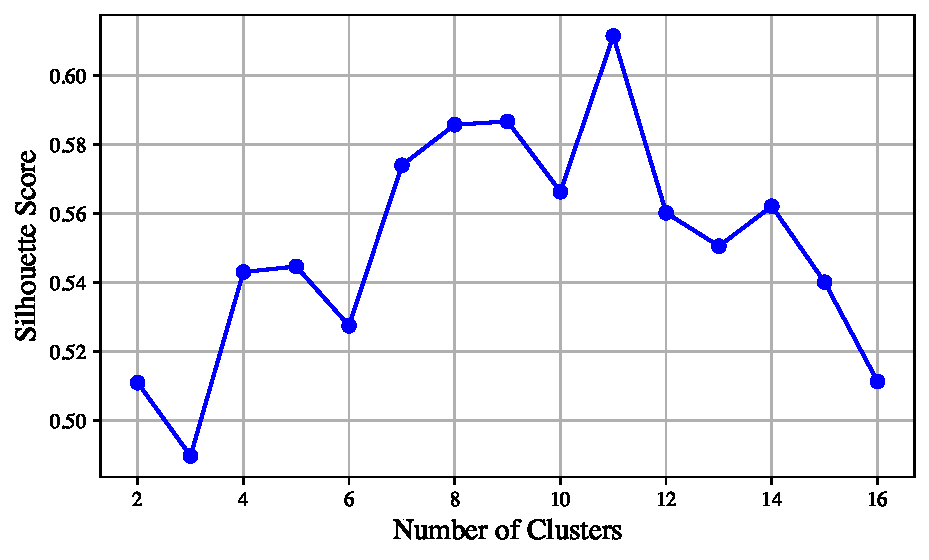
\includegraphics[width=\columnwidth]{figures/silhouette_11.pdf} 
    \caption{Silhouette scores for the numbers of clusters}
    \label{fig:silhouette}
\end{figure}

As can be seen in figure \ref{fig:kmeans}, the data was separated into 9 different clusters. A small blue dot depicts each cluster center. As can be seen in figure \ref{fig:silhouette}, for a maximum number of $n=10$, the 

\begin{figure}[htbp]
    \centering
    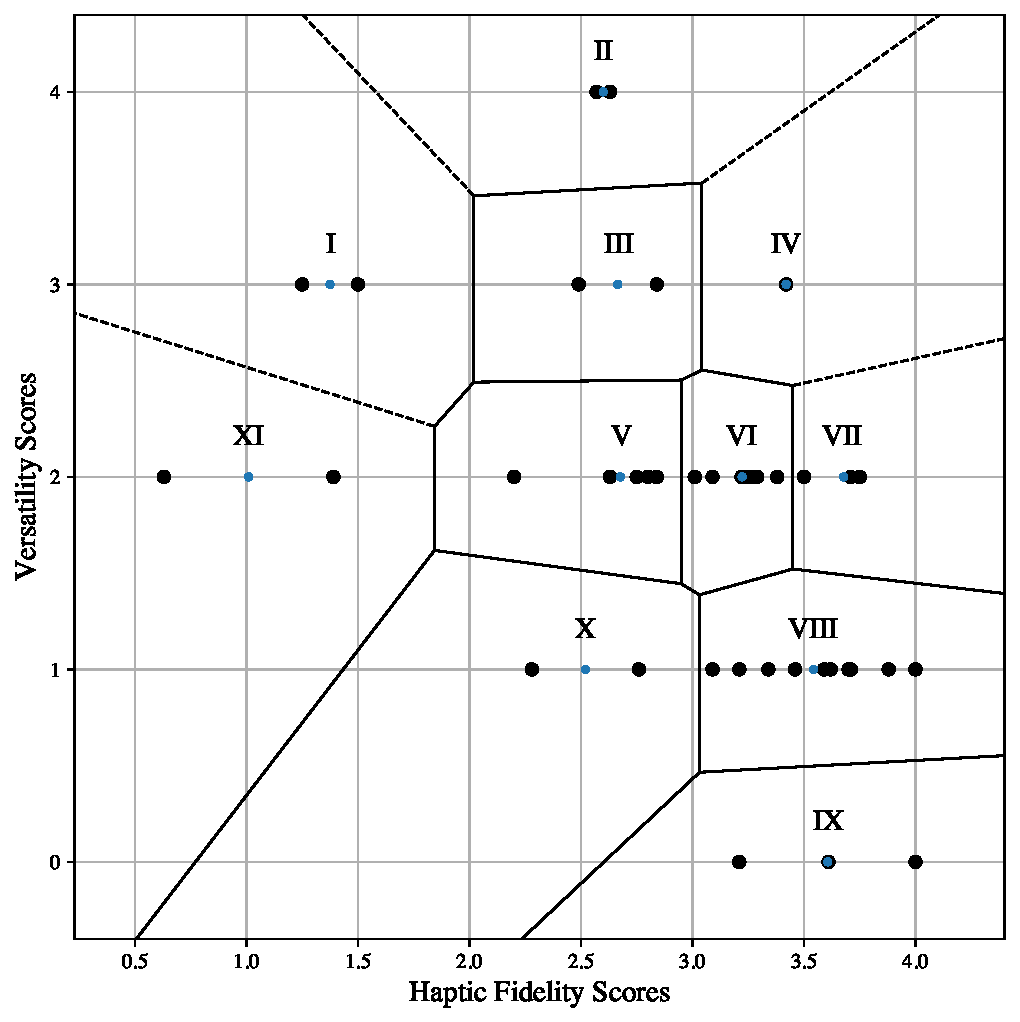
\includegraphics[width=\columnwidth]{figures/k_means_11.pdf} 
    \caption{K-means clustering of the data, n=11}
    \label{fig:kmeans}
\end{figure}

\begin{figure}[htbp]
    \centering
    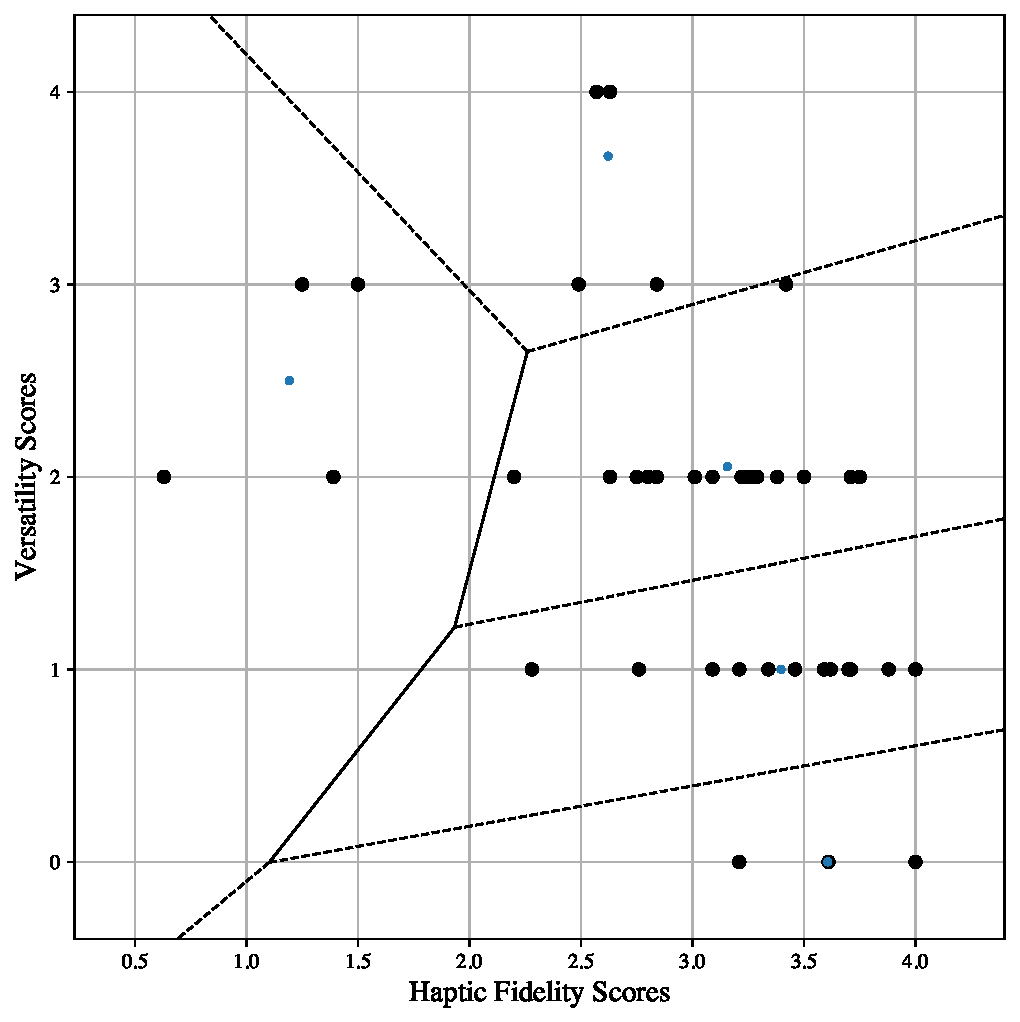
\includegraphics[width=\columnwidth]{figures/k_means_5.pdf} 
    \caption{K-means clustering of the data, n=5}
    \label{fig:kmeans}
\end{figure}



\subsubsection{Evaluation of the clusters}
% Explain each cluster, describe differences and similarities

\textbf{Cluster I} contains the articles by Hanashima et al. and H. Liu et al. \cite{Hanashima2023, LiuH2019}. Both systems have a relatively high versatility score, the haptic feedback however is rather abstract. The haptic feedback is exclusively generated through vibration. While the system developed by Hanashima et al. provides haptic feedback on the head and the waist to help the participants with posture learning, H. Liu et al. developed a glove-based system that gives feedback when grasping and lifting virtual objects. While H. Liu found a significantly improved success rate when grasping the objects under the condition of the haptic feedback, Hanashima et al. found the visual feedback only condition to be superior over the visuo-tactile condition. 


